\documentclass[11pt,a4paper]{article}

% ---------------------------------------------------------------------------
% MedSkel AI -- rapport de projet (module Réseaux de Neurones et Apprentissage Profond)
% Compilation : latexmk -pdf rapport_medskel_ai.tex
% Les figures de figures/private/ contiennent des images FIVES (CC BY 4.0) :
% elles ne sont pas versionnées (règle du dépôt) mais sont nécessaires à la compilation.
% ---------------------------------------------------------------------------

\usepackage[T1]{fontenc}
\usepackage[utf8]{inputenc}
\usepackage[french]{babel}
\usepackage{lmodern}
\usepackage{microtype}
\usepackage[margin=2.4cm]{geometry}
\usepackage{amsmath,amssymb,bm,mathtools}
\usepackage{icomma}
\usepackage{booktabs,tabularx,multirow}
\usepackage{graphicx}
\usepackage{caption}
\usepackage{xcolor}
\usepackage{tikz}
\usetikzlibrary{arrows.meta,positioning,calc}
\usepackage{enumitem}
\usepackage{fancyhdr}
\usepackage{titlesec}
\usepackage[hidelinks]{hyperref}

\definecolor{teal}{HTML}{0F8B8D}
\definecolor{ink}{HTML}{1E2A33}
\definecolor{soft}{HTML}{EEF6F6}
\definecolor{warn}{HTML}{B5532A}

\titleformat{\section}{\Large\bfseries\color{teal}}{\thesection}{0.6em}{}
\titleformat{\subsection}{\large\bfseries\color{ink}}{\thesubsection}{0.6em}{}
\captionsetup{font=small,labelfont=bf}
\setlist{itemsep=1pt,topsep=3pt}
\pagestyle{fancy}
\fancyhf{}
\fancyhead[L]{\small\color{teal}MedSkel AI}
\fancyhead[R]{\small Rapport de projet -- Réseaux de Neurones et Apprentissage Profond}
\fancyfoot[C]{\small\thepage}
\renewcommand{\headrulewidth}{0.3pt}
\newcommand{\pct}{\,\%}

\begin{document}

% ---------------------------------------------------------------------------
\begin{titlepage}
\centering
{\large École d'Ingénierie Digitale et d'Intelligence Artificielle (EIDIA)\par}
{\large Université Euromed de Fès\par}
\vspace{2.6cm}
{\Huge\bfseries\color{teal} MedSkel AI\par}
\vspace{0.5cm}
{\LARGE Segmentation des vaisseaux rétiniens par U-Net\\[2pt] et mesure géométrique des vaisseaux\par}
\vspace{1.4cm}
\begin{tikzpicture}[node distance=0.45cm, every node/.style={font=\small}]
  \tikzstyle{stp}=[rectangle,rounded corners=3pt,draw=teal,fill=soft,minimum width=2.2cm,minimum height=1.0cm,align=center]
  \node[stp] (a) {Photo\\du fond d'œil};
  \node[stp,right=of a] (b) {U-Net :\\masque des vaisseaux};
  \node[stp,right=of b] (c) {MedSkel :\\lignes centrales};
  \node[stp,right=of c] (d) {Mesures\\(pixels)};
  \node[stp,right=of d] (e) {Comparaison\\sains / malades};
  \foreach \x/\y in {a/b,b/c,c/d,d/e} \draw[-{Stealth},thick,teal] (\x) -- (\y);
\end{tikzpicture}
\vspace{2cm}

{\large Rapport de projet\par}
{Module : Réseaux de Neurones et Apprentissage Profond\par}
{Enseignant : Pr. N. Joudar\par}
\vfill
{\Large Mouhssine El Boumshouli\par}
{4\textsuperscript{e} année, cycle ingénieur\par}
\vspace{0.4cm}
{Novembre 2026\par}
{\small Code : \url{https://github.com/MouhssineElBoumshouli/medskel-ai}\par}
\end{titlepage}

% ---------------------------------------------------------------------------
\section*{Résumé}
Nous entraînons un réseau U-Net en PyTorch, sans poids pré-entraînés (7\,849\,601 paramètres), pour marquer les vaisseaux sanguins dans des photographies du fond d'œil. Les données proviennent du jeu public FIVES (800 images de $2048\times2048$ pixels annotées par des experts, quatre groupes : sain, DMLA, rétinopathie diabétique, glaucome). L'entraînement se fait sur un GPU portable de 4\,Go, par tuiles de $512\times512$ pixels. Toutes les décisions sont prises sur un jeu de validation séparé ; le jeu de test officiel n'est utilisé qu'à la fin.

Le modèle final atteint un \textbf{Dice moyen de 0,889} (intervalle à 95\pct : 0,873 -- 0,903) sur les 200 images de test de FIVES. Un U-Net avec encodeur ResNet34 pré-entraîné, utilisé comme référence, atteint 0,907. Sur un jeu externe d'une autre caméra (CHASE\_DB1, 28 images de 14 enfants), notre modèle atteint un Dice de 0,766 face au premier expert, contre 0,777 pour le second expert humain ; il marque cependant plus de pixels que les experts. La faiblesse principale est la détection des vaisseaux les plus fins (rappel de 0,46).

Nous relions ensuite le réseau à la méthode géométrique MedSkel (lignes centrales par bissectrices, Saidou et al., 2024) pour mesurer les vaisseaux. Avec MedSkel, le nombre de bifurcations varie deux fois moins qu'avec l'amincissement classique lorsque le masque de l'expert est remplacé par celui du réseau (26\pct contre 53\pct). Les yeux atteints de DMLA, de rétinopathie diabétique ou de glaucome présentent une densité vasculaire, une dimension fractale, une longueur totale et un nombre de bifurcations plus faibles que les yeux sains ($p<0{,}001$). Ces mesures ne suffisent toutefois pas à classer un œil individuel (exactitude équilibrée de 0,45 à 0,49 pour 4 groupes). Il s'agit d'un outil de recherche, pas d'un dispositif de diagnostic.

\tableofcontents
\newpage

% ---------------------------------------------------------------------------
\section{Introduction}

\subsection{Contexte}
La rétine est le seul endroit du corps où l'on peut observer des vaisseaux sanguins de façon non invasive, par simple photographie du fond d'œil. La forme de ces vaisseaux (densité, calibre, ramifications, tortuosité) est étudiée en recherche car elle est associée à des maladies oculaires et générales : rétinopathie diabétique, glaucome, hypertension. Une étude récente sur 10\,151 participants sains de la UK Biobank a ainsi relié 114 caractéristiques vasculaires à l'âge, à la pression artérielle, à l'IMC et à l'HbA1c \cite{yusufu}.

Avant de mesurer, il faut \textbf{trouver} les vaisseaux, pixel par pixel. C'est un problème de \textbf{segmentation sémantique} : pour chaque pixel, décider s'il appartient à un vaisseau. Le tracé manuel par un expert est lent, et deux experts ne tracent pas exactement la même chose.

\subsection{Point de départ}
Un projet antérieur, \texttt{medskel}, implémente une méthode géométrique d'extraction de lignes centrales inspirée de Saidou et al.\ \cite{saidou}. Son point faible était la première étape : les vaisseaux y étaient détectés par un filtre classique (filtre de Frangi), peu fiable. Ce projet remplace ce filtre par un réseau de neurones convolutif, puis réutilise MedSkel pour mesurer.

\subsection{Objectifs et contributions}
\begin{enumerate}
  \item Construire et expliquer un U-Net complet en PyTorch, entraîné de zéro sur de vraies annotations (FIVES).
  \item L'évaluer honnêtement : séparation stricte entraînement / validation / test, intervalles de confiance, test externe sur un autre jeu de données et comparaison avec un second expert humain.
  \item Identifier la faiblesse principale (les vaisseaux fins) et tester des améliorations une par une.
  \item Relier le masque du réseau à MedSkel pour obtenir des mesures, et vérifier leur stabilité et leur lien avec les groupes de maladies.
  \item Livrer une application locale qui enchaîne toutes les étapes.
\end{enumerate}

% ---------------------------------------------------------------------------
\section{Données}

\subsection{FIVES}
FIVES \cite{fives} contient 800 photographies couleur du fond d'œil (caméra TRC-NW8, champ de 50°, $2048\times2048$ pixels) de 573 patients, avec un masque binaire des vaisseaux tracé par des experts. Les images se répartissent en quatre groupes de 200 : DMLA (A), rétinopathie diabétique (D), glaucome (G) et sain (N). Les auteurs définissent 600 images d'entraînement et 200 de test.

Nous avons d'abord audité les données (script \texttt{python -m medskel\_ai.data}) :
\begin{itemize}
  \item 800 paires image/masque de même nom et de même taille ; masques strictement binaires (0 et 255) ;
  \item les vaisseaux couvrent en moyenne 7,5\pct\ des pixels (N : 9,0\pct ; A : 7,3\pct ; D : 6,9\pct ; G : 6,7\pct) ;
  \item \textbf{2 masques entièrement noirs} dans l'entraînement (447\_G, 448\_G) : erreurs d'annotation, exclus ;
  \item \textbf{6 paires de photographies identiques} octet par octet (5 dans l'entraînement, 1 dans le test, aucune entre les deux) : chaque paire est gardée du même côté de la séparation.
\end{itemize}

\textbf{Séparation.} Des 598 images d'entraînement utilisables, 88 forment la validation (22 par groupe, graine 42) et 510 servent à l'entraînement. La même séparation est utilisée dans toutes les expériences.

\begin{center}
\begin{tabular}{@{}lcl@{}}
\toprule
\textbf{Ensemble} & \textbf{Images} & \textbf{Rôle} \\
\midrule
Entraînement & 510 & apprentissage des poids \\
Validation & 88 & toutes les décisions (seuil, arrêt, choix des expériences) \\
Test (officiel) & 200 & score final uniquement \\
\bottomrule
\end{tabular}
\end{center}

\subsection{CHASE\_DB1 (test externe)}
CHASE\_DB1 \cite{chase} contient 28 photographies (les deux yeux de 14 enfants), prises avec une autre caméra (Nidek NM-200-D, 30°, $999\times960$ pixels). Chaque image a \textbf{deux} masques tracés indépendamment par deux observateurs, ce qui permet de mesurer l'accord entre deux humains. Aucune image CHASE n'a servi à entraîner, choisir un modèle ou fixer un seuil.

\subsection{Limite}
Les 800 images FIVES proviennent de 573 patients et aucun identifiant patient n'est publié : deux photographies d'un même patient peuvent se trouver de part et d'autre de la séparation. Les scores portent donc sur des \emph{images} jamais vues, pas sur des \emph{patients} prouvés jamais vus.

% ---------------------------------------------------------------------------
\section{Méthode : le réseau U-Net}

\subsection{Convolution}
Une couche de convolution fait glisser un petit filtre appris sur l'image. Pour une entrée $X$ à $C$ canaux et un filtre $W$ de taille $3\times3$, la sortie au pixel $(i,j)$ est
\begin{equation}
Y(i,j) \;=\; b \;+\; \sum_{c=1}^{C}\sum_{u=-1}^{1}\sum_{v=-1}^{1} W(c,u,v)\; X(c,\,i+u,\,j+v).
\end{equation}
Exemple : le filtre $\begin{psmallmatrix}-1&2&-1\\-1&2&-1\\-1&2&-1\end{psmallmatrix}$ répond $3\times(2\times9)=54$ sur une ligne verticale de valeur 9, et $0$ sur une ligne horizontale ou une zone uniforme : c'est un détecteur de lignes verticales. Les poids $W$ et le biais $b$ ne sont pas choisis à la main : ils sont \textbf{appris}. Chaque couche utilise plusieurs filtres, chacun produisant une \emph{carte de caractéristiques}. Un rembourrage (\emph{padding}) de zéros garde la taille de l'image.

\subsection{Non-linéarité, normalisation et sous-échantillonnage}
\begin{itemize}
  \item \textbf{ReLU} : $\mathrm{ReLU}(x)=\max(0,x)$. Sans elle, une suite de convolutions resterait une seule opération linéaire.
  \item \textbf{Normalisation par lots} (\emph{batch normalisation}) \cite{bn} : chaque canal est recentré et remis à l'échelle,
  $\hat{x} = \gamma\,\frac{x-\mu_B}{\sqrt{\sigma_B^2+\varepsilon}} + \beta$, ce qui stabilise et accélère l'apprentissage.
  \item \textbf{Max pooling} $2\times2$ : on garde le maximum de chaque bloc de $2\times2$. La carte est deux fois plus petite ; les filtres suivants voient une zone plus grande de l'image (le contexte nécessaire pour distinguer un vaisseau d'une tache sombre), au prix de la position exacte.
\end{itemize}

\subsection{Architecture}
Le U-Net \cite{unet} est un encodeur--décodeur symétrique (figure~\ref{fig:unet}).
\begin{itemize}
  \item \textbf{Encodeur} : 4 blocs de 32, 64, 128 et 256 canaux. Chaque bloc = (convolution $3\times3$, normalisation, ReLU) $\times 2$, puis max pooling.
  \item \textbf{Goulot} : 512 canaux, à $32\times32$ pixels pour une tuile de $512\times512$.
  \item \textbf{Décodeur} : 4 étapes de suréchantillonnage bilinéaire $\times2$, puis \textbf{concaténation} avec la carte de l'encodeur de même taille (\emph{connexion de saut}), puis un bloc de convolutions.
  \item \textbf{Sortie} : une convolution $1\times1$ donne un \emph{logit} $z$ par pixel ; la sigmoïde $\sigma(z)=1/(1+e^{-z})$ le transforme en probabilité.
\end{itemize}
Les connexions de saut sont essentielles : le décodeur sait \emph{ce qui} est présent (information profonde), et les cartes de l'encodeur rapportent \emph{où} précisément (information fine). Sans elles, les vaisseaux fins disparaissent. Le réseau compte \textbf{7\,849\,601 paramètres}, tous appris à partir de zéro.

\begin{figure}[h]
\centering
\begin{tikzpicture}[x=1cm,y=1cm,font=\scriptsize]
  \tikzstyle{blk}=[rectangle,draw=teal,fill=soft,minimum height=0.5cm,minimum width=2.4cm,align=center,rounded corners=2pt]
  \node[blk,fill=white] (in) at (0,1) {tuile $512^2\times3$};
  \node[blk] (e1) at (0,0)    {$512^2$, 32};
  \node[blk] (e2) at (0.6,-0.9) {$256^2$, 64};
  \node[blk] (e3) at (1.2,-1.8) {$128^2$, 128};
  \node[blk] (e4) at (1.8,-2.7) {$64^2$, 256};
  \node[blk,fill=teal!20] (b) at (4.4,-3.6) {$32^2$, 512};
  \node[blk] (d4) at (7.0,-2.7) {$64^2$, 256};
  \node[blk] (d3) at (7.6,-1.8) {$128^2$, 128};
  \node[blk] (d2) at (8.2,-0.9) {$256^2$, 64};
  \node[blk] (d1) at (8.8,0)  {$512^2$, 32};
  \node[blk,fill=green!15] (out) at (8.8,1) {probabilité / pixel};
  \draw[-{Stealth}] (in) -- (e1);
  \foreach \a/\b in {e1/e2,e2/e3,e3/e4,e4/b} \draw[-{Stealth}] (\a) -- node[left]{\tiny pool} (\b);
  \foreach \a/\b in {b/d4,d4/d3,d3/d2,d2/d1} \draw[-{Stealth}] (\a) -- node[right]{\tiny up} (\b);
  \draw[-{Stealth}] (d1) -- node[right]{\tiny conv $1{\times}1$ + $\sigma$} (out);
  \foreach \a/\b in {e1/d1,e2/d2,e3/d3,e4/d4} \draw[-{Stealth},dashed,warn] (\a.east) -- (\b.west);
\end{tikzpicture}
\caption{Architecture U-Net utilisée (taille spatiale, nombre de canaux). Flèches pointillées : connexions de saut (concaténation).}
\label{fig:unet}
\end{figure}

% ---------------------------------------------------------------------------
\section{Méthode : apprentissage}

\subsection{Fonction de perte}
Soit $y_k\in\{0,1\}$ la vérité et $p_k=\sigma(z_k)$ la probabilité prédite au pixel $k$, sur $N$ pixels.

\textbf{Entropie croisée binaire} (calculée directement sur les logits pour la stabilité numérique) :
\begin{equation}
\mathcal{L}_{\text{BCE}} = -\frac{1}{N}\sum_{k}\Big[y_k\ln p_k + (1-y_k)\ln(1-p_k)\Big].
\end{equation}
Pour un pixel de vaisseau, $p=0{,}9$ coûte $-\ln 0{,}9\approx0{,}11$, alors que $p=0{,}1$ coûte $-\ln0{,}1\approx2{,}30$ : les erreurs confiantes sont fortement pénalisées.

\textbf{Perte de Dice douce} \cite{vnet} :
\begin{equation}
\mathcal{L}_{\text{Dice}} = 1-\frac{2\sum_k p_k y_k + \epsilon}{\sum_k p_k + \sum_k y_k + \epsilon}.
\end{equation}
Comme seulement 7,5\pct\ des pixels sont des vaisseaux, la BCE seule est dominée par le fond. La perte de Dice ne regarde que le recouvrement des vaisseaux et compense ce déséquilibre. Nous utilisons $\mathcal{L}=\mathcal{L}_{\text{BCE}}+\mathcal{L}_{\text{Dice}}$ (poids égaux).

\subsection{Rétropropagation et optimisation}
La rétropropagation calcule le gradient $\nabla_\theta\mathcal{L}$ par rapport à chacun des 7,8 millions de paramètres, en appliquant la règle de dérivation en chaîne couche par couche, de la sortie vers l'entrée. Les paramètres sont mis à jour par \textbf{Adam} \cite{adam}, avec $g_t=\nabla_\theta\mathcal{L}$ :
\begin{align}
m_t &= \beta_1 m_{t-1} + (1-\beta_1)\,g_t, \qquad v_t = \beta_2 v_{t-1} + (1-\beta_2)\,g_t^2,\\
\theta_t &= \theta_{t-1} - \eta_t\,\frac{\hat m_t}{\sqrt{\hat v_t}+\epsilon}, \qquad \hat m_t=\frac{m_t}{1-\beta_1^t},\;\; \hat v_t=\frac{v_t}{1-\beta_2^t}.
\end{align}
$m_t$ est une moyenne des gradients récents (inertie), $v_t$ adapte le pas à chaque paramètre. Le taux d'apprentissage $\eta_t$ part de $10^{-3}$ et décroît jusqu'à 0 selon un cosinus sur un budget de temps fixé.

\subsection{Protocole d'entraînement}
\begin{itemize}
  \item \textbf{Tuiles} : un GPU de 4\,Go (RTX 3050 portable) ne peut pas traiter une image de $2048\times2048$ ; réduire l'image ferait disparaître les vaisseaux fins. Chaque pas utilise 4 tuiles aléatoires de $512\times512$ à pleine résolution (2 images $\times$ 2 tuiles).
  \item \textbf{Augmentation} : symétries, rotations de 90°, petites variations de luminosité et de contraste.
  \item \textbf{Précision mixte}, graine fixe (42). Après chaque époque, le Dice sur des tuiles fixes de validation sélectionne les meilleurs poids.
\end{itemize}

\subsection{Prédiction}
Une image entière est découpée en tuiles de $512\times512$ qui se chevauchent de 64 pixels ; les probabilités sont moyennées dans les zones de chevauchement. Option \textbf{symétries au test} (TTA) : l'image est prédite 4 fois (originale, miroir gauche--droite, haut--bas, les deux), chaque résultat est remis dans le bon sens et les 4 cartes sont moyennées. Le seuil de décision est choisi sur la validation.

% ---------------------------------------------------------------------------
\section{Protocole d'évaluation}

À partir des comptes de pixels VP, FP, FN, VN (vrais/faux positifs/négatifs) de chaque image :
\begin{gather*}
\text{Dice}=\frac{2\,VP}{2\,VP+FP+FN},\qquad
\text{IoU}=\frac{VP}{VP+FP+FN},\\[4pt]
\text{Précision}=\frac{VP}{VP+FP},\qquad
\text{Rappel}=\frac{VP}{VP+FN},\qquad
\text{Spécificité}=\frac{VN}{VN+FP}.
\end{gather*}
Les scores sont calculés par image puis moyennés.

\textbf{Pourquoi pas l'exactitude ?} Une prédiction entièrement noire obtient une exactitude de 0,929 sur le test FIVES avec un Dice de 0 : l'exactitude est trompeuse quand une classe est rare.

\textbf{Deux métriques ciblées sur la faiblesse :}
\begin{itemize}
  \item \textbf{clDice} \cite{cldice} mesure la connectivité : on compare les squelettes (lignes de 1 pixel) des deux masques, de sorte qu'un vaisseau fin compte autant, par unité de longueur, qu'un vaisseau épais, et qu'un vaisseau interrompu est pénalisé.
  \item \textbf{Rappel sur vaisseaux fins} : proportion des pixels de vaisseaux de 1 à 4 pixels de large (largeur locale estimée par la transformée de distance sur le squelette expert) retrouvés par le modèle. Ces pixels ne représentent que 1,7\pct\ des pixels de vaisseaux, donc le Dice ne les « voit » presque pas.
\end{itemize}

\textbf{Intervalles de confiance} : bootstrap à 10\,000 tirages des images (des \emph{enfants} pour CHASE, car les deux yeux d'un enfant ne sont pas indépendants).

\textbf{Règles fixées à l'avance} : (1) toute décision se prend sur la validation ; (2) un seul changement à la fois, même graine, même séparation ; (3) le test FIVES n'est évalué qu'une fois les choix figés --- il a été utilisé pour la version 1 puis pour la version finale, soit deux fois au total ; (4) CHASE est évalué avec le modèle et le seuil fixés sur FIVES.

% ---------------------------------------------------------------------------
\section{Résultats de segmentation}

\subsection{Version 1 (référence)}
Après 50 minutes d'entraînement (38 époques), le seuil choisi sur la validation est 0,40. Sur le test FIVES : Dice $0{,}875\pm0{,}114$ (écart type), intervalle à 95\pct\ 0,858 -- 0,890, médiane 0,907 ; IoU 0,791 ; précision 0,909 ; rappel 0,856 ; spécificité 0,993.

\subsection{Mesurer la faiblesse}
Sur la validation, ce modèle retrouve 89,5\pct\ des pixels des vaisseaux épais, mais \textbf{seulement 45,9\pct\ des pixels des vaisseaux fins} (intervalle 42,2 -- 49,7\pct).

\subsection{Expériences (validation uniquement)}
\begin{table}[h]
\centering\small
\begin{tabular}{@{}lccccl@{}}
\toprule
\textbf{Expérience} & \textbf{Seuil} & \textbf{Dice} & \textbf{clDice} & \textbf{Rappel fins} & \textbf{Retenue ?} \\
\midrule
Référence (50 min) & 0,40 & 0,8985 & 0,9048 & 0,459 & -- \\
E1 : + symétries au test & 0,35 & 0,9017 & 0,9091 & 0,480 & oui \\
E2 : entraînement de 150 min & 0,25 & 0,9072 & 0,9126 & 0,487 & oui \\
E3 : + perte clDice (50 min) & 0,35 & 0,8901 & 0,8986 & 0,438 & \textbf{non} \\
E4 : E2 + symétries (final) & 0,30 & \textbf{0,9100} & \textbf{0,9154} & 0,484 & final \\
\bottomrule
\end{tabular}
\caption{Validation, 88 images. Gain de E4 sur la référence : +0,011 de Dice (intervalle 0,009 -- 0,014).}
\label{tab:exp}
\end{table}
L'entraînement plus long (115 époques, figure~\ref{fig:curves}) et les symétries au test améliorent les trois métriques. La perte clDice, testée avec un seul poids et un budget de 50 minutes, dégrade tout, y compris le clDice : elle a été abandonnée (« inutile dans nos conditions », et non « inefficace en général »).

\begin{figure}[h]
\centering
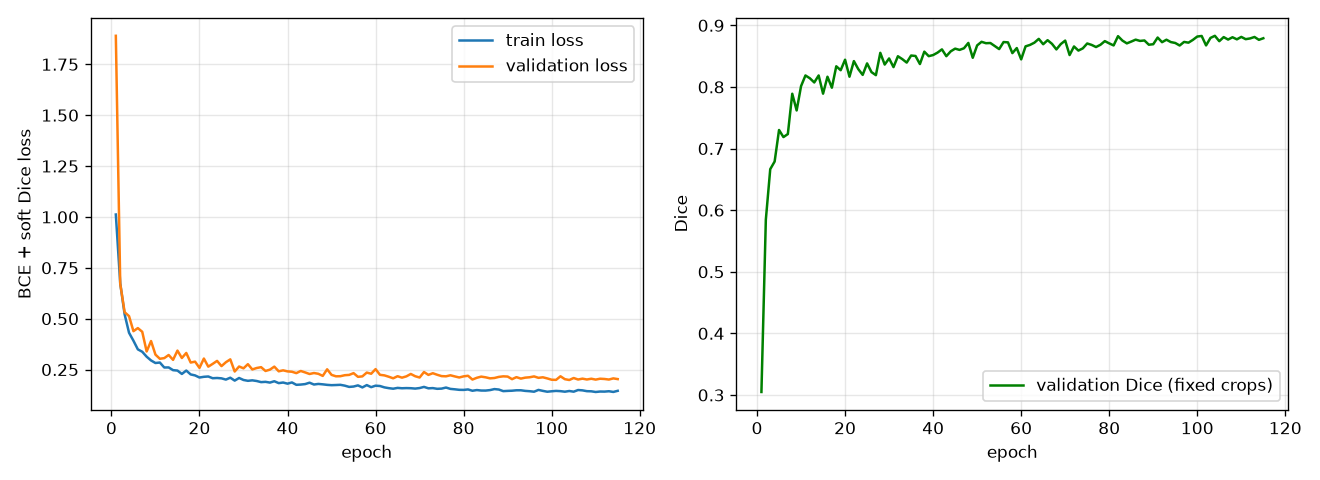
\includegraphics[width=0.92\textwidth]{figures/curves_final.png}
\caption{Modèle final (E2) : pertes d'entraînement et de validation (gauche) et Dice de validation (droite) par époque. La perte de validation ne remonte pas : pas de surapprentissage marqué.}
\label{fig:curves}
\end{figure}

\subsection{Test final sur FIVES}
\begin{table}[h]
\centering\small
\begin{tabular}{@{}lccccc@{}}
\toprule
\textbf{Métrique} & \textbf{Tous (200)} & \textbf{DMLA} & \textbf{Rétino. diab.} & \textbf{Glaucome} & \textbf{Sain} \\
\midrule
Dice & \textbf{0,889} (0,873 -- 0,903) & 0,917 & 0,888 & 0,850 & 0,902 \\
clDice & 0,897 (0,881 -- 0,911) & 0,921 & 0,895 & 0,851 & 0,921 \\
Précision & 0,919 & 0,934 & 0,935 & 0,916 & 0,891 \\
Rappel & 0,874 & 0,906 & 0,854 & 0,820 & 0,917 \\
\bottomrule
\end{tabular}
\caption{Test FIVES du modèle final. IoU 0,813 ; spécificité 0,994 ; médiane du Dice 0,914 ; rappel sur vaisseaux fins 0,458. Gain sur la version 1 : +0,015 (0,012 -- 0,017).}
\end{table}

\begin{figure}[h]
\centering
\includegraphics[width=\textwidth]{figures/private/example_67D.png}\\[2pt]
\includegraphics[width=\textwidth]{figures/private/example_4A.png}
\caption{Deux images de test FIVES : photographie, masque expert, prédiction, superposition (prédiction en vert). Images FIVES, Jin et al.\ 2022, licence CC BY 4.0.}
\end{figure}

\textbf{Référence pré-entraînée.} Un U-Net à encodeur ResNet34 \cite{resnet} pré-entraîné sur ImageNet (24,4 millions de paramètres, même données et même budget) atteint un Dice de \textbf{0,907} (0,891 -- 0,921). Il est meilleur sur toutes les métriques, ce qui est attendu : il démarre avec des filtres appris sur 1,2 million d'images et il est trois fois plus grand. Notre modèle est une base saine et entièrement explicable, pas le meilleur modèle possible.

\subsection{Test externe sur CHASE\_DB1 et comparaison avec un humain}
\begin{table}[h]
\centering\small
\begin{tabular}{@{}lcccc@{}}
\toprule
\textbf{Comparaison (contre l'observateur 1)} & \textbf{Dice} & \textbf{clDice} & \textbf{Sensibilité} & \textbf{Spécificité} \\
\midrule
Notre modèle final & 0,766 & 0,835 & 0,908 & 0,949 \\
Modèle pré-entraîné & 0,770 & 0,840 & 0,914 & 0,949 \\
\textbf{Observateur 2 (humain)} & \textbf{0,777} & 0,835 & 0,769 & 0,978 \\
\bottomrule
\end{tabular}
\caption{CHASE\_DB1, 28 images de 14 enfants, jamais utilisées pour l'entraînement ni pour un choix. Les images CHASE sont agrandies d'un facteur $\approx1{,}31$ pour avoir le même nombre de pixels par degré que FIVES.}
\end{table}
\begin{itemize}
  \item Le Dice chute de 0,889 (FIVES) à 0,766 (CHASE) ; même deux experts ne s'accordent qu'à 0,777 sur ce jeu.
  \item Le modèle commet des erreurs d'une autre nature que l'humain : sensibilité bien plus haute (+0,139, intervalle 0,103 -- 0,176) et précision plus basse (0,66 contre 0,80). Il marque \textbf{plus} de pixels que les experts.
  \item Les gains de la version 2 et l'avantage du modèle pré-entraîné disparaissent sur CHASE : la limite vient du changement de caméra et de population, pas de la taille du modèle.
\end{itemize}

\subsection{Les pires images}
Les trois pires images ont été examinées à l'œil. Pour \texttt{train/174\_D} (validation, Dice 0,15), le masque expert \textbf{ne correspond pas à la photographie} : erreur d'annotation du jeu de données (figure~\ref{fig:worst}). Les deux pires images de test (\texttt{122\_G}, \texttt{123\_G}) sont des photographies très sombres et floues où l'expert n'a tracé que quelques segments.

\begin{figure}[h]
\centering
\includegraphics[width=0.75\textwidth]{figures/private/worst_174D.png}
\caption{\texttt{train/174\_D} : photographie, masque expert, prédiction. L'arbre vasculaire du masque expert ne correspond pas à celui de la photographie ; la prédiction suit les vaisseaux visibles.}
\label{fig:worst}
\end{figure}

% ---------------------------------------------------------------------------
\section{Du masque à la mesure : MedSkel}

\subsection{Lignes centrales}
Pour mesurer la longueur d'un vaisseau ou compter ses bifurcations, il faut sa ligne centrale (squelette). Deux méthodes sont comparées :
\begin{itemize}
  \item \textbf{Amincissement} (méthode standard, \texttt{scikit-image}) : on retire les pixels du bord, couche par couche, jusqu'à une ligne d'un pixel. Simple, mais sensible aux petites irrégularités du contour, qui deviennent de petites branches parasites.
  \item \textbf{MedSkel} \cite{saidou} : le contour est approché par un polygone (simplification à $\varepsilon=4$ px), puis la ligne centrale est formée des points équidistants des deux bords, calculés par diagramme de Voronoï. Le code du projet \texttt{medskel} d'origine est importé en lecture seule.
\end{itemize}

\textbf{Mesures} (en pixels ; aucune conversion validée en millimètres) : densité vasculaire (part du champ rétinien couverte), dimension fractale (par comptage de boîtes : pente de $\log N(s)$ contre $\log(1/s)$), longueur totale, nombre de bifurcations, largeur médiane, tortuosité médiane. La tortuosité dépend trop de la méthode (environ 1,07 avec l'amincissement à cause de l'effet d'escalier, 1,01 avec MedSkel à cause de la simplification) : elle n'est pas interprétée.

\textbf{Correction d'un biais.} Dans le code MedSkel d'origine, la largeur d'une branche n'est calculée qu'aux sommets conservés après simplification, surtout situés aux extrémités, où le vaisseau s'affine : un vaisseau test de 12 pixels de large est mesuré à 1,3 pixel. Sans modifier le dépôt d'origine, la largeur est ici mesurée de la même manière pour les deux méthodes (transformée de distance le long de la ligne centrale). Les résultats de \emph{longueur} du projet d'origine ne sont pas concernés.

\textbf{Vérification.} Entre les deux observateurs de CHASE, la longueur totale varie de 9,3\pct\ (amincissement) et 3,2\pct\ (MedSkel) : exactement les valeurs du projet d'origine, ce qui valide le branchement des deux codes.

\subsection{Stabilité des mesures}
La différence relative entre deux mesures $a$ et $b$ est $|a-b|/\frac{a+b}{2}$.
\begin{table}[h]
\centering\small
\begin{tabular}{@{}lcc|cc@{}}
\toprule
 & \multicolumn{2}{c|}{\textbf{FIVES test : CNN vs expert}} & \multicolumn{2}{c}{\textbf{CHASE : humain 2 vs humain 1}} \\
\textbf{Mesure} & Amincissement & MedSkel & Amincissement & MedSkel \\
\midrule
Densité vasculaire & 0,057 & (même masque) & 0,127 & (même masque) \\
Longueur totale & 0,068 & 0,063 & 0,093 & 0,032 \\
Bifurcations & 0,532 & \textbf{0,258} & 0,216 & 0,122 \\
Largeur médiane & 0,178 & \textbf{0,133} & 0,175 & 0,173 \\
\bottomrule
\end{tabular}
\caption{Différence relative médiane (plus bas = plus stable). FIVES : 200 images, test de Wilcoxon $p<0{,}001$ pour les quatre mesures de squelette.}
\end{table}

Sur FIVES, remplacer le masque expert par celui du réseau change la densité et la longueur d'environ 6 à 7\pct. Avec MedSkel, le nombre de bifurcations varie \textbf{deux fois moins} qu'avec l'amincissement. Sur CHASE en revanche, les mesures du réseau s'écartent plus des experts que les experts entre eux (densité : 0,302 contre 0,127 ; largeur : 0,39 à 0,67 contre 0,17), conséquence directe du sur-marquage observé à la section précédente (figure~\ref{fig:chase}).

\begin{figure}[h]
\centering
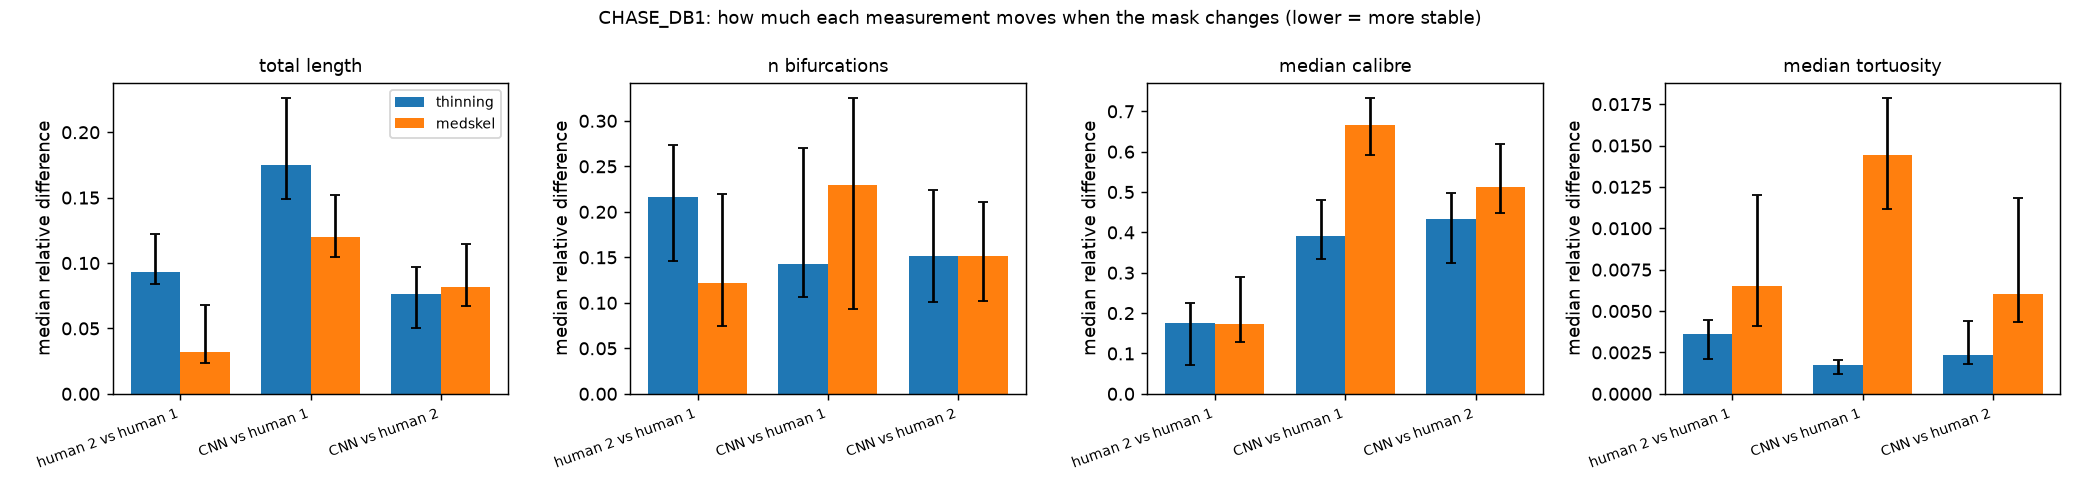
\includegraphics[width=\textwidth]{figures/chase_agreement.png}
\caption{CHASE\_DB1 : différence relative médiane de chaque mesure entre humain 2 et humain 1, et entre le réseau et chaque humain, pour les deux méthodes de squelette.}
\label{fig:chase}
\end{figure}

\subsection{Mesures et groupes de maladies}
\begin{table}[h]
\centering\small
\begin{tabular}{@{}lcccc@{}}
\toprule
\textbf{Mesure (médiane)} & \textbf{Sain (200)} & \textbf{DMLA (194)} & \textbf{Rétino. diab. (199)} & \textbf{Glaucome (198)} \\
\midrule
Densité vasculaire & 11,6\pct & 10,0\pct & 9,6\pct & 9,4\pct \\
Dimension fractale & 1,528 & 1,501 & 1,497 & 1,490 \\
Longueur totale (px) & 30\,435 & 26\,620 & 23\,732 & 25\,159 \\
Bifurcations & 177 & 138 & 142 & 155 \\
\bottomrule
\end{tabular}
\caption{Masques experts FIVES (entraînement + test, doublons comptés une fois, masques erronés exclus), amincissement. Kruskal--Wallis $p<0{,}001$ pour chaque mesure ; chaque maladie contre sain : Mann--Whitney corrigé de Holm, $p<0{,}001$.}
\end{table}

Les trois groupes malades présentent une densité vasculaire, une dimension fractale, une longueur totale et un nombre de bifurcations plus faibles que les yeux sains. Le même schéma apparaît avec les masques du réseau sur les 200 images de test (figure~\ref{fig:groups}).

\begin{figure}[h]
\centering
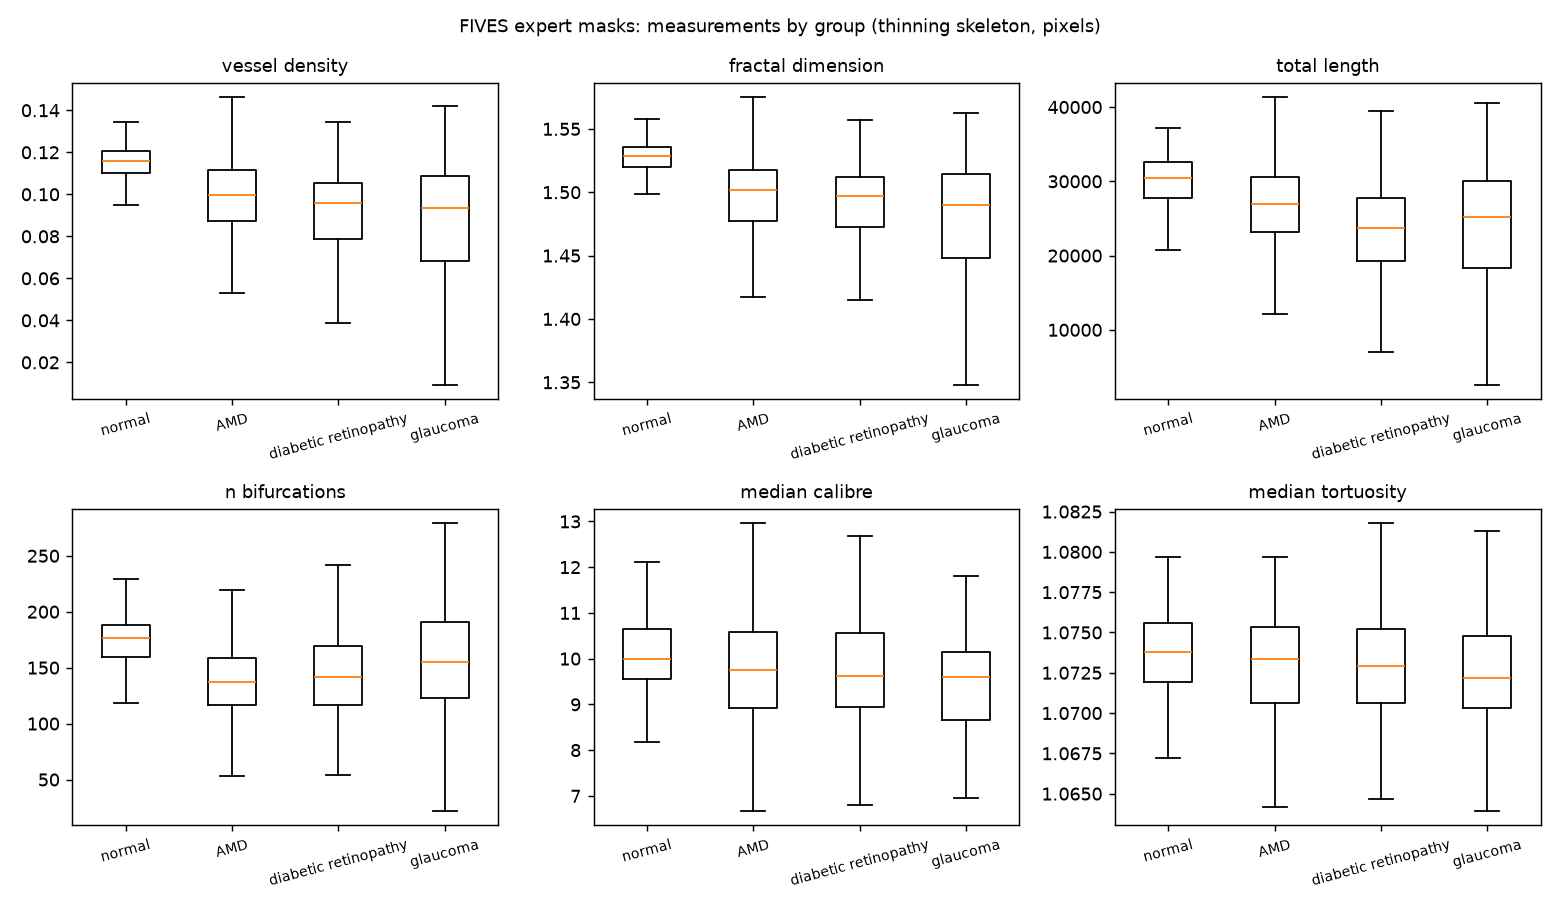
\includegraphics[width=0.95\textwidth]{figures/groups_expert.png}
\caption{Distribution des mesures par groupe (masques experts FIVES, amincissement, pixels).}
\label{fig:groups}
\end{figure}

\textbf{Classer un œil à partir des mesures ?} Une régression logistique sur les 6 mesures, entraînée sur les images d'entraînement et évaluée une fois sur les 200 images de test :
\begin{center}\small
\begin{tabular}{@{}llcc@{}}
\toprule
\textbf{Lignes centrales} & \textbf{Masques de test} & \textbf{Exactitude équilibrée (hasard : 0,25)} & \textbf{AUC sain vs RD} \\
\midrule
Amincissement & experts & 0,488 & 0,818 \\
Amincissement & réseau & 0,449 & 0,842 \\
MedSkel & experts & 0,457 & 0,748 \\
MedSkel & réseau & 0,453 & 0,805 \\
\bottomrule
\end{tabular}
\end{center}
Avec des étiquettes mélangées, l'exactitude moyenne est de 0,251 ($p\le0{,}004$) : les mesures portent une information réelle, et la chaîne complète photo $\to$ réseau $\to$ mesures fonctionne presque aussi bien qu'avec les masques experts. Mais le classifieur se trompe plus d'une fois sur deux. Comme dans la littérature \cite{yusufu}, le lien est net \textbf{à l'échelle des groupes} et trop faible \textbf{pour un individu}. Il s'agit d'associations dans un seul jeu de données, qui peuvent aussi refléter la qualité des images, des lésions masquant des vaisseaux, ou la façon dont les experts annotent les yeux malades.

% ---------------------------------------------------------------------------
\section{Application}
Une application locale (Gradio) enchaîne toutes les étapes : chargement d'une photographie, segmentation (curseur avant/après), lignes centrales MedSkel, tableau des mesures et graphique de position de l'œil par rapport aux 4 groupes (figure~\ref{fig:app}). Chaque mesure est comparée à 50 yeux sains du test FIVES traités exactement de la même façon (réseau puis MedSkel). Les mesures sont exportables en CSV. L'application affiche clairement qu'il ne s'agit pas d'un diagnostic, et ne propose volontairement aucune prédiction de maladie individuelle. Elle se lance par un double clic (\texttt{MedSkel AI.bat}) ; une analyse complète prend environ 6 secondes sur le GPU portable.

\begin{figure}[h]
\centering
\begin{minipage}{0.47\textwidth}\centering\includegraphics[width=\textwidth]{figures/private/app_top.png}\end{minipage}\hfill
\begin{minipage}{0.5\textwidth}\centering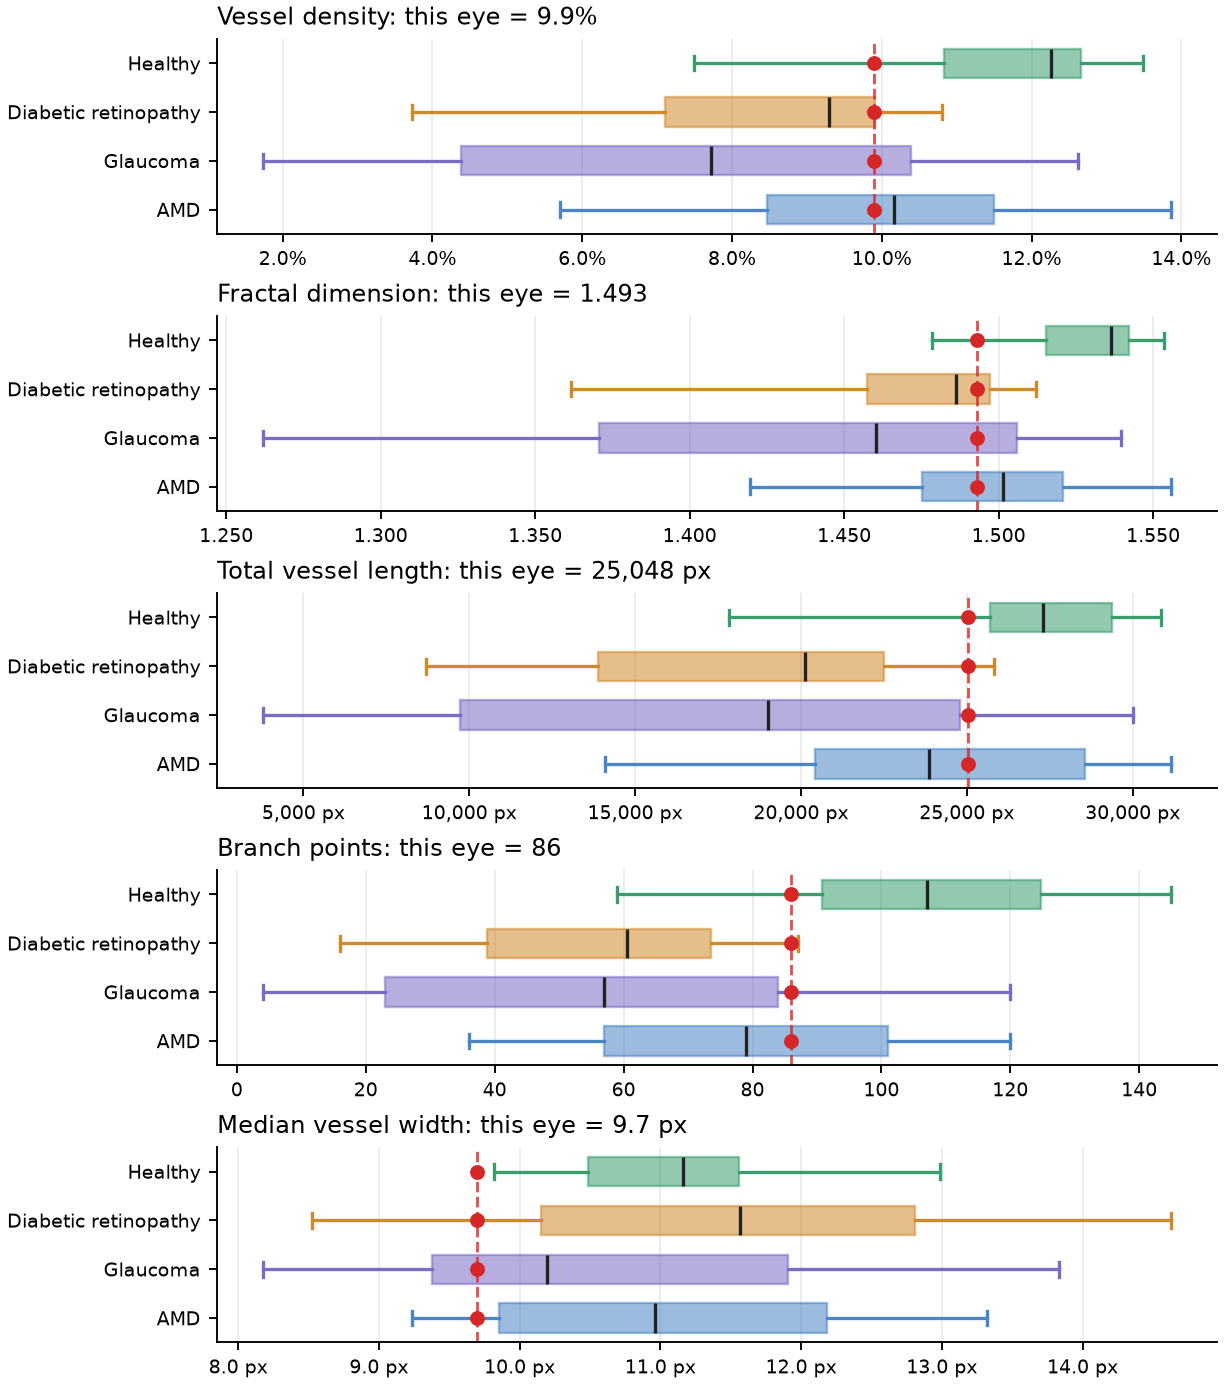
\includegraphics[width=\textwidth]{figures/eye_chart.png}\end{minipage}
\caption{Gauche : l'application (vaisseaux en vert, lignes centrales MedSkel en rouge). Droite : position d'un œil de test (point rouge) par rapport aux 4 groupes FIVES ; les distributions se chevauchent largement.}
\label{fig:app}
\end{figure}

% ---------------------------------------------------------------------------
\section{Discussion et limites}
\begin{itemize}
  \item \textbf{Vaisseaux fins} : environ 46\pct\ seulement des pixels des vaisseaux de 1 à 4 pixels sont retrouvés ; ni l'entraînement plus long ni la perte clDice ne l'ont résolu.
  \item \textbf{Généralisation} : sur une autre caméra (CHASE), le Dice baisse et le réseau sur-marque ; les mesures ne sont pas encore transférables.
  \item \textbf{Unités} : mesures en pixels uniquement.
  \item \textbf{Patients} : l'indépendance patient entre entraînement et test n'est pas garantie dans FIVES.
  \item \textbf{Variabilité} : un seul entraînement par configuration (une graine) ; de très petites différences ne doivent pas être sur-interprétées.
  \item \textbf{Test réutilisé} : le test FIVES a été évalué deux fois (version 1 et version finale), toujours après avoir figé les choix.
  \item \textbf{Usage clinique} : aucun. Ce n'est pas un dispositif médical.
\end{itemize}

% ---------------------------------------------------------------------------
\section{Conclusion et perspectives}
Un U-Net de 7,8 millions de paramètres, entraîné de zéro sur un GPU portable, segmente les vaisseaux rétiniens de FIVES avec un Dice de 0,889 et atteint, sur un jeu externe, un accord proche de celui de deux experts entre eux. Relié à la méthode géométrique MedSkel, il fournit des mesures plus stables qu'avec l'amincissement classique, et ces mesures reproduisent des différences connues entre yeux sains et malades, sans permettre de diagnostic individuel.

Perspectives : améliorer les vaisseaux fins (perte pondérée par l'épaisseur, résolution plus fine), adapter le modèle à d'autres caméras (augmentation de domaine, données supplémentaires), calibrer une échelle en millimètres, répéter les entraînements avec plusieurs graines, et, à plus long terme, valider les mesures avec des données cliniques en partenariat avec un service d'ophtalmologie.

% ---------------------------------------------------------------------------
\appendix
\section{Code et reproduction}
Le code est en Python/PyTorch : \url{https://github.com/MouhssineElBoumshouli/medskel-ai}. Les données et les poids ne sont pas versionnés.
\begin{center}\small
\begin{tabularx}{\textwidth}{@{}lX@{}}
\toprule
\textbf{Fichier} & \textbf{Rôle} \\
\midrule
\texttt{src/medskel\_ai/data.py} & audit de FIVES, appariement image/masque, séparation, tuiles \\
\texttt{src/medskel\_ai/model.py} & le U-Net \\
\texttt{src/medskel\_ai/train.py} & entraînement (BCE + Dice, Adam, précision mixte) \\
\texttt{src/medskel\_ai/predict.py} & prédiction par tuiles, symétries au test \\
\texttt{src/medskel\_ai/evaluate.py} & métriques, choix du seuil, bootstrap \\
\texttt{src/medskel\_ai/chase.py} & test externe CHASE\_DB1 \\
\texttt{src/medskel\_ai/morphometry.py} & lignes centrales et mesures \\
\texttt{src/medskel\_ai/study.py} & étude des mesures (stabilité, groupes, classifieur) \\
\texttt{app.py}, \texttt{MedSkel AI.bat} & application \\
\texttt{tests/} & tests automatiques (pytest) sur données synthétiques \\
\bottomrule
\end{tabularx}
\end{center}
\begin{verbatim}
python -m medskel_ai.train --minutes 150          # entraînement
python -m medskel_ai.evaluate --split val         # choix du seuil
python -m medskel_ai.evaluate --split test        # test final (une fois)
python -m medskel_ai.study all                    # étude des mesures
python app.py                                     # application
\end{verbatim}

% ---------------------------------------------------------------------------
\begin{thebibliography}{99}\small
\bibitem{unet} O. Ronneberger, P. Fischer, T. Brox. \emph{U-Net: Convolutional Networks for Biomedical Image Segmentation}. MICCAI, 2015.
\bibitem{fives} K. Jin et al. \emph{FIVES: A Fundus Image Dataset for Artificial Intelligence based Vessel Segmentation}. Scientific Data 9, 475, 2022. doi:10.1038/s41597-022-01564-3.
\bibitem{chase} M. M. Fraz et al. \emph{An Ensemble Classification-Based Approach Applied to Retinal Blood Vessel Segmentation}. IEEE Trans. Biomedical Engineering 59, 2012.
\bibitem{saidou} N. Saidou et al. \emph{A Novel Method of Skeletonization of Complex Shapes Based on Bisectors}. 2024. doi:10.1142/S2972370123500083.
\bibitem{cldice} S. Shit et al. \emph{clDice -- a Novel Topology-Preserving Loss Function for Tubular Structure Segmentation}. CVPR, 2021.
\bibitem{vnet} F. Milletari, N. Navab, S.-A. Ahmadi. \emph{V-Net: Fully Convolutional Neural Networks for Volumetric Medical Image Segmentation}. 3DV, 2016.
\bibitem{adam} D. P. Kingma, J. Ba. \emph{Adam: A Method for Stochastic Optimization}. ICLR, 2015.
\bibitem{bn} S. Ioffe, C. Szegedy. \emph{Batch Normalization: Accelerating Deep Network Training by Reducing Internal Covariate Shift}. ICML, 2015.
\bibitem{resnet} K. He, X. Zhang, S. Ren, J. Sun. \emph{Deep Residual Learning for Image Recognition}. CVPR, 2016.
\bibitem{yusufu} M. Yusufu et al. \emph{Population-Based Normative Reference for Retinal Microvascular Atlas}. Ophthalmology Science, 2025. doi:10.1016/j.xops.2025.100723.
\end{thebibliography}

\end{document}
